
\subsection*{task 1.4 \\[1ex] getting used to slicing (part 1)}

Read image \texttt{asterix.png} into an array \texttt{arrF} and image \texttt{portrait.png} into an array \texttt{arrG}.

Now, create a copy \texttt{arrH} of \texttt{arrF} and then ---without using \keyword{for} loops--- paste \texttt{arrG} into \texttt{arrH} such that the upper left corner of \texttt{arrG} is at array coordinate $[i,j] = [100, 200]$ in \texttt{arrH}. Write your result as a PNG image.

To illustrate how this image should look like, here is the result you would obtain from using $[i,j] = [10, 10]$
%%%%%
%%%%%
%%%%% enter your result here, i.e. replace "t1-4.png" by the name of your resulting image file
%%%%%
%%%%%
\begin{center}
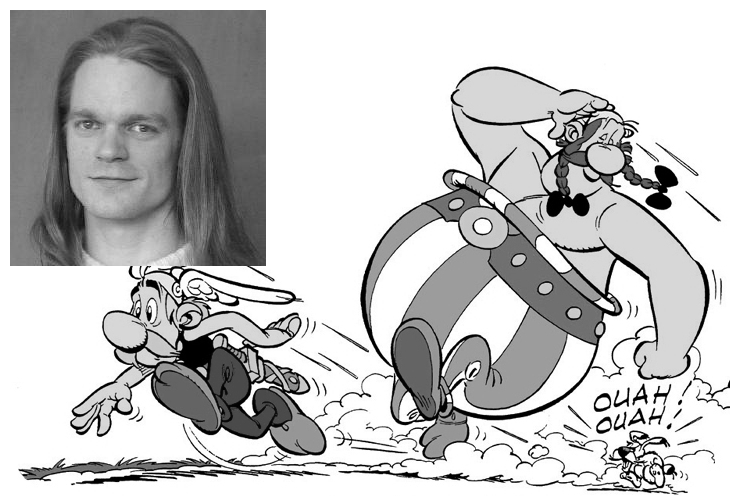
\includegraphics[width=0.5\textwidth]{t1-4.png} 
\end{center}
%%%%%
%%%%%
%%%%%
%%%%%
%%%%%
Simply replace the above image with the image you just created.






